\part{Apprentissage automatique par la pratique}
\pagebreak

\chapter{Rappel}
\section{Matrices et calcules sur les Matrices}

\subsection{Addition}

$\left(\begin{array}{cc}
1 & 3 \\ 1 & 0 \\ 1 & 2 \end{array} \right)$
+
$\left(\begin{array}{cc}
0 & 0 \\ 7 & 5 \\ 2 & 1 \end{array} \right) $
=
$\left(\begin{array}{cc}
1+0 & 3+0 \\ 1+7 & 0+5 \\ 1+2 & 2+1 \end{array} \right) $
=
$\left(\begin{array}{cc}
1 & 3 \\ 8 & 5 \\ 3 & 3 \end{array} \right) $

\subsection{Multiplication}

$\begin{array}{c@{\ }c}
&
\left(\begin{array}{cc}
5 & 6 \\ 7 & 8 \end{array} \right) \\[0.5cm]
\left(\begin{array}{cc}
1 & 2 \\ 3 & 4 \end{array} \right)
&
\left(\begin{array}{cc}
19 & 22 \\ 43 & 50 \end{array} \right)
\end{array}$

$(1 * 5) + (2 * 7) = 19$

\subsection{Transposer}

$\left(\begin{array}{ccc}
1 & 3 & 5 \\ 2 & 4 & 6 \end{array} \right) $
= 
$\left(\begin{array}{cc}
1 & 2 \\ 3 & 4 \\ 5 & 6 \end{array} \right) $

\subsection{Inverse}
\begin{description}
\item[Soit une matrice 2x2 comme]:
$\left(\begin{array}{ccc}
a & b \\ c & d \end{array} \right) $
\item[Soit Determinant D] = ad - bc
\item[Si D != 0 alors il existe une matrice inverse égal à]:
$ \frac{1}{D} \left(\begin{array}{ccc}
d & -b \\ -c & a \end{array} \right) $
\end{description}

\chapter{Algorithms Learn a Mapping From Input to Output}
\section{linear ML algorithms}

\begin{description}
\item[] Simplifier les processus d'apprentissage et réduire la fonction sur ce qu'on connait
\item[Soit ]: B0 + B1X1 + B2X2 + B3X3 = 0
\item[] Où B0,B1,B2,B3 sont les coefficients présent sur l'axe des ordonnées.
\item[] Et X1,X2,X3 sont les valeurs en Input.
\end{description}

\section{Supervised machine learning}
L'apprentissage supervisé peut se diviser en 2 partis
\begin{description}
\item[Classification]: Quand les variables en sortie sont des Classe $(Vert, Carre, Homme)$
\item[Regression]: Quand les variables en sortie sont des valeur numérique $(euro, poids, quantites)$
\end{description}

\section{Unsupervised machine learning}
Les problèmes de l'apprentissage non supervisé sont:
\begin{description}
\item[Clustering]: L'art de faire des paquet d'éléments qui ont des points commun, comme regrouper les clients par paquet de choses qu'ils ont le plus en commun.
\item[Association]: Associer des règles d'apprentissage pour décrire une portion du data, comme une personne qui a acheté un item A et qui est aussi tenté par acheter un item B
\end{description}

\section{semi-supervised machine leaning}
L'apprentissage semi supervisé c'est avoir un bonne quantité de données en input X, et un peu de data avec le label Y.

\section{Overview of dias and variance}
La prédiction des erreurs pour les algorithmes sont regroupé en 3 points:
\begin{description}
\item[Bias Error]:  Simplifier l'hypothèse fait par le modèls pour faire une fonction d'apprentissage plus facile.
\item[Variance Error]: Et la quantité estimé par la fonction visé qui changera via un différent ensemble de data utilisé.
\item[Irreductible Error]: Ne peut pas être réduit
\end{description}

\chapter{Overfitting and Underfitting}
\section{Overfitting}
L'overfitting intervient lorsque le modèle sur apprend des connaissances,
Lorsque l'on sur apprend nous prenons en compte les points plus éloigné de la droite de la fonction.\\
On peut illustrer l'overfitting en codant un algorithme qui prend en compte les points bleu et rouges de la figure $\textit{ap-linear-regression\_1}$ ce dessous.\\

\section{Underfitting}
C'est l'inverse de l'overfitting, pas assez de données pour pouvoir généraliser le base de connaissance.\\
\pagebreak

\chapter{Model Selection}
\pagebreak
\section{Train Test Split}
S'applique à de très gros dataset.\\
Sépare les listes $xset$ et $yset$ en $train,\ test$ sous liste.\\
Les ensemble de retours $xtrain,ytrain$ et $xtest,ytest$ ont le même nombres de lignes et la taille.\\
La taille des ensembles $test$ sont une proportion de la taille du $set$ multiplié par la paramètre $text_size$.\\

\lstset{style=mlpythoncode}
\begin{lstlisting}[language=Python]
from sklearn.model_selection import train_test_split

xtrain, xtest, ytrain, ytest = train_test_split(xset, yset, test_size=0.1, random_state=0)
\end{lstlisting}

\funcdoc{sklearn.model\_selection.train\_test\_split}{
\begin{description}
\item[xset,yset] Souvent de type $\cblue{pandas.DataFrame}$.
\item[test\_size] $\paramtype{float btw 0 \& 1}$ le nombre de rows que $xtest,ytest$ contiendra en proportion de la taille des entrées.
\item[random\_state] $\paramtype{Integer}$ la graine utilisé pour les générateurs de nombre aléatoire.
\item[shuffle] $\paramtype{Boolean}$ Mélanger ou pas les sets avant la séparation.
\end{description}
}{
\begin{description}
\item[arrays] 
\end{description}
}{}
\pagebreak
\section{Cross validation}
S'applique à un jeu de donné de taille moyenne.\\
La séparation d'un jeu de donnée d'entrainement et de test peuvent donner par hasard des jeux de données non représentatifs.\\
Pour éviter ce cas, il est nécessaire de reproduire plusieurs fois la procédure puis de moyenner les résultats retournée.\\
Chaque étape de la cross validation va retournée 2 ensemble (respectivement égaux au indices de $train,test$:\\

\lstset{style=mlpythoncode}
\begin{lstlisting}[language=Python]
from sklearn.model_selection import KFold

kf = KFold(n_splits=10, shuffle=True)
for trainI, testI in kf.split(xset):
    xtrain, xtest = xset[trainI], xset[testI]
    ytrain, ytest = yset[trainI], yset[testI]
\end{lstlisting}
\ \\
Exemple simple d'un instance $\cblue{KFold}(n\_split=3, shuffle=False)$ sur un dataSet de taille 15.\\
Les éléments en rouge seront les éléments sélectionné dans les ensembles de $test$ et les éléments en noir seront les $train$:\\
\begin{description}
\item[k=1] $\crouge{A}$,$\crouge{B}$,$\crouge{C}$,$\crouge{D}$,$\crouge{E}$,F,G,H,I,J,K,L,M,N,O
\item[k=2] A,B,C,D,E,$\crouge{F}$,$\crouge{G}$,$\crouge{H}$,$\crouge{I}$,$\crouge{J}$,K,L,M,N,O
\item[k=3] A,B,C,D,E,F,G,H,I,J,$\crouge{K}$,$\crouge{L}$,$\crouge{M}$,$\crouge{N}$,$\crouge{O}$
\end{description}

\funcdoc{sklearn.model\_selection.KFold}{
\begin{description}
\item[n\_split] $\paramtype{Integer}$ Nombre de split à effectuer
\item[shuffle] $\paramtype{Boolean}$ Mélanger ou pas les sets avant la séparation.
\end{description}
}{
\begin{description}
\item[arrays] 
\end{description}
}{}

\section{Leave one out}
S'applique à des dataset de petite taille.\\
Pour chaque item du dataset, le prendre en tant que $test$ et le reste en tant que $train$.\\

\lstset{style=mlpythoncode}
\begin{lstlisting}[language=Python]
from sklearn.model_selection import LeaveOneOut
loo = LeaveOneOut()

for train_index, test_index in loo.split(X):
   X_train, X_test = X[train_index], X[test_index]
   y_train, y_test = y[train_index], y[test_index]
\end{lstlisting}


\pagebreak

\section{Matrice de confusion, Précision, Pecall, F1}
Tout ces paramètres indique la consistance de la dataSet, ils sont calculé via une matrice de confusion:\\
\lstset{style=mlpythoncode}
\begin{lstlisting}[language=Python]
from sklearn.metrics import confusion_matrix
print(confusion_matrix(ytrain, ypredicted))
>> array([[tn,  fp],
          [fn,  tp]])
          
tn, fp, fn, tp = confusion_matrix(ytrain,ypredicted).ravel()
\end{lstlisting}

\funcdoc{sklearn.metrics.confusion\_matrix}{
\begin{description}
\item[y\_true] $\paramtype{array}$ les y valides.
\item[y\_pred] $\paramtype{array}$ les y qui ont était prédit via un classifier.
\end{description}
}{
\begin{description}
\item[arrays] 
\end{description}
}{
\begin{description}
\item[ravel()] $\paramtype{arrays}$ retourne les index dans l'ordre de leurs position:
\begin{description}
\item[tn] les vrai négatifs
\item[fp] les faux positifs 
\item[fn] les faux négatifs
\item[tp] les vrai positifs
\end{description}
\end{description}
}

Les Précision, Recall, F1 peuvent être calculé depuis le tableau de sortie qu'offre $\cblue{confusion\_matrix}$, mais il existe des méthodes permettent de le faire à notre place:\\

\lstset{style=mlpythoncode}
\begin{lstlisting}[language=Python]
from sklearn.metrics import precision_recall_fscore_support

prf = precision_recall_fscore_support(ytest, ypredicted)
print(zip(["Precision", "Recal", "F1", "Support"], [numpy.mean(row) for row in prf]))
{"Precision": _, "Recal": _, "F1": _, "Support": _}
\end{lstlisting}

\funcdoc{sklearn.metrics.precision\_recall\_fscore\_support}{
\begin{description}
\item[y\_true] $\paramtype{array}$ les y valides.
\item[y\_pred] $\paramtype{array}$ les y qui ont était prédit via un classifier.
\end{description}
}{
\begin{description}
\item[arrays] 
\end{description}
}{}

\chapter{Linear Algorithms}
Soit X l'ensemble des variables indépendantes sur l'axe des l'abscisse et
Y l'ensemble des variable dépendantes sur l'axe des ordonnée.

\section{Régression linéaire}
Étant donné un plan à deux dimensions où l'abscisse contient les point d'entrée X et l'ordonnée contient les points de sortie Y, et un nouage de points précédaient acquitté de tout point éloigné du nuage.\\

\scalebox{0.7}{
\begin{tikzpicture}
  \begin{axis} [
      xlabel     = X, % label x axis
      ylabel     = Y, % label y axis
      axis lines = left, %set the position of the axes
      clip       = false, 
      xmin       = 0,
      ymin       = 0,
    ]
    \addplot [color=black] coordinates { (0,0)(10,10) };
    \addplot [only marks, mark=*, color=blue] coordinates {(1,2)(2.5,3)(5,6)(4,3)(8,9)(6,4)(3,4)(7,6) };
    \addplot [only marks, mark=*, color=red] coordinates {(1,9)(8,1)(9,1.5) };
  \end{axis}
\end{tikzpicture}
}
\begin{description}
\item[Avec]: y  = $\beta_0 + \beta_1 x$
\item[Pour un hyperPlan (3d)]: y = $\beta_0 + \beta_1 x_1 + \beta_2 x_2$
\item[$P-I_n$]: y = $\beta_0 + \beta_1 x_1 + ... \beta_n x_n$
\end{description}
\lstset{style=mlpythoncode}
\begin{lstlisting}[language=Python]
from sklearn.linear_model import LinearRegression

reg = LinearRegression().fit(xtrain, ytrain)
reg.score(xtest, ytest)
reg.predict(xtest)
\end{lstlisting}

\funcdoc{sklearn.linear\_model.LinearRegression}{}{}{
\begin{description}
\item[fit(X,y)] $\paramtype{pandas.DataFrame}$ Apprend le modèle avec les data $X$ et $y$.
\item[predict(X)] $\paramtype{pandas.DataFrame}$ Test l'apprentissage avec les données $X$ et retourne le $y$ généré.
\item[score(X,y)] $\paramtype{pandas.DataFrame}$ Retourne le coefficient de prédiction en comparent les $y$ généré avec le $y$ en paramètre.
\end{description}
}

\pagebreak
\section{Least squares linear regression}
Calculer la régression linéaire avec la méthode Least squares:\\
Soit:
\begin{description}
\item[X] = $[1,2,3,4,5]$ les variables indépendantes d'axe abscisse
\item[Y] = $[2,4,5,4,5]$ les variables dépendantes d'axe ordonnée
\item[Calculons] $y = \beta_0 + \beta_1 x$
\end{description}
\ \\
Calcule de la moyenne de X et Y:
\begin{description}
\item[Xm] = $ \sum x_i \in X$ = 3
\item[Ym] = $ \sum y_i \in Y$ = 4
\end{description}
\ \\
Toutes ligne de régression doivent passer par le point (Xm,Ym).\\
Calculer tout les écarts des $x_i \in X$ par rapport à Xm (resp Y):\\

\begin{tabular}{ll|l|l|l|l}
  \hline
  X  & Y & $X - Xm$ & $Y - Ym$ & $(X-Xm)^2$ & $(X-Xm)(Y-Ym)$\\
  \hline
  1 & 2 & -2 & -2 & 4 & 4\\
  2 & 4 & -1 & 0  & 1 & 0\\
  3 & 5 & 0  & 1  & 0 & 0\\
  4 & 4 & 1  & 0  & 1 & 0\\
  5 & 5 & 2  & 1  & 4 & 2\\ 
  \hline
\end{tabular}

\begin{description}
\item[$Calculer \beta_1$]:
\item[$ \beta_1 $] = $ \frac{ \sum (X-Xm)(Y-Ym)}{ \sum (X-Xm)^2}$ = $\frac{6}{10}$ = $.6$
\item[$ \beta_0 $]: $Ym = \beta_0 + \beta_1 * Xm$ : $4 = \beta_0 + .6 * 3$ : $4= \beta_0 + 1.8$ : $\beta_0 = 2.2$
\end{description}
\pagebreak
\section{Gradient Descent}
Soit:
\begin{description}
\item[X] = $[1,2,4,3,5]$
\item[Y] = $[1,3,3,2,5]$
\item[i] = une variable qui itère les éléments de X et Y en bouclant à l'infini.
\end{description}
Une initialisation comme:
\begin{description}
\item[$\beta_0$] = 0
\item[$\beta_1$] = 0
\item[$\alpha$] = donnée en énoncé (pour l'exemple égal à 0.01)
\end{description}
Et des fonctions définit tel que:
\begin{description}
\item[error] = $(\beta_0 + \beta_1 * X[i]) - Y[i]$
\item[$\beta_{0_{+1}}$] = $\beta_0 - \alpha * error$
\item[$\beta_{1_{+1}}$] = $\beta_1 - \alpha * error * X[i]$
\end{description}

En appliquant l'algorithme des calcules des $\beta_i$:\\
\begin{tabular}{l|l|l|l|l|l}
  \hline
  $ i $ & $ X[i] $ &  $Y[i] $ &  $error $ & $ \beta_0 $ & $ \beta_1 $\\
  \hline
  0 & 1 & 1 & -1 & 0.01 & 0.01 \\
  1 & 2 & 3 & -2.97 & 0.06 & 0.03\\
  2 & 4 & 3 & -1.77 & 0.18 & 0.06\\
  3 & 3 & 2 & -1.61 & 0.22 & 0.08\\
  4 & 5 & 5 & -4.35 & 0.44 & 0.12\\
  0 & 1 & 1 & -0.42 & 0.45 & 0.13\\
  1 & 2 & 3 & -2.28 & 0.49 & 0.49\\
  \hline
\end{tabular}
\pagebreak
\section{Logistic Regression}
\subsection{Logistic function}

Soit:
\begin{description}
\item[t] $\in \Re[0,1]$ égal à $\beta_0 + \beta_2 * x$
\end{description}

La fonction de logique de régression, les valeur d'entrée X sont combiné en utilisant les coefficient de valeur pour prédire une sortie Y. Cette sortie sera une valeur binaire.

\begin{description}
\item[$p(x)$] = $ \frac{1}{1 + e^{-(P-I_n)}}$
\item[Note]: $p(x)$ peut être interprété comme une fonction de probabilité $P(X) = P[Y=1 | X)$.
\item[$\beta_0 + \beta_1 * x$] = $ ln(\frac{P(x)}{1 - P(x)})$ aussi appelé odds.
\end{description}

\lstset{style=mlpythoncode}
\begin{lstlisting}[language=Python]
from sklearn.linear_model import LogisticRegression

c = LogisticRegression().fit(xtrain,ytrain)
c.predict(xtest)
c.score(xtest, ytest)
\end{lstlisting}

\funcdoc{sklearn.linear\_model.LogisticRegression}{}{}{
\begin{description}
\item[fit(X,y)] $\paramtype{pandas.DataFrame}$ Apprend le modèle avec les data $X$ et $y$.
\item[predict(X)] $\paramtype{pandas.DataFrame}$ Test l'apprentissage avec les données $X$ et retourne le $y$ généré.
\item[score(X,y)] $\paramtype{pandas.DataFrame}$ Retourne le coefficient de prédiction en comparent les $y$ généré avec le $y$ en paramètre.
\end{description}
}

\section{Linear Discriminant Analysis}
L'analyse discriminante linéaire fait partie des techniques d'analyse discriminante prédictive, il s'agit de prédire l'appartenance d'un individu à une classe prédéfinie à partir de ses caractéristiques mesurées à l'aide de variables prédictives.\\
A notre disposition, un échantillon de $n$ observations réparties dans $\Bbbk$ groupes d'effectifs $n_{\Bbbk}$.\\
\begin{description}
\item[Noté $Y$] les variables prédire $\{y1, ... y_{\Bbbk}\}$
\item[$J$] variables prédictives $X = (X_1, ... X_j)$
\item[$\mu_{\Bbbk}$] la moyenne (ou $\textit{mean}$ en anglais) valant $lambda(list) -> \frac{\sum list[i]}{taille(list)}$
\item[$\sigma^2$] la variance de toutes les classes $\frac{\sum_{i=1}^n (x_i - \mu_{\Bbbk})^2}{n - \Bbbk}$
\item[la fonction discriminante pour la classe $\Bbbk$ avec $x$ donné] $D_{\Bbbk} (x) = x * \frac{\mu_{\Bbbk}}{\omega^2} - \frac{\mu_{\Bbbk}^2}{2x\omega^2} + ln(P(k))$
\item[Où $P(k)$] vaut la probabilité appliqué aux valeurs de $Y$
\end{description}

\subsection{bayésien rules}
L'objectif est de produire une règle d'affection $X(\omega) \rightarrow Y(\omega)$ qui permet de prédire, pour une observation $\omega$ donné, sa valeur associé de $Y$ à partir des valeurs prises par $X$. via une probabilité\\
\begin{description}
\item[$P(Y=y_{\Bbbk})$] = $\frac{P(Y=y_{Bbbk})*P(X|Y=y_{\Bbbk})}{\sum_{i=1}^{\Bbbk} P(Y=y_i)*P(X|Y=y_i)}$
\item[Où $P(Y=y_{\Bbbk})$] est la probabilité à $priori$ d'appartenance à une classe
\item[$P(X|Y=y_{\Bbbk})$] représente la fonction de densité des X conditionnellement à la classe $y_{\Bbbk}$
\end{description}

\chapter{Non linear algorithm}
\section{Classification and régression tree}
Soit:\\
\begin{description}
\item[$G$] $ = \sum_{k=1}^n p_k * (1 - p_k)$
\item[$V$] = 2.67
\item[] \begin{tabular}{ll|l}
  \hline
  $ X_1 $ & $ X_2 $ &  $Y $\\
  \hline
  2.77 & 2.33 & 0\\
  1.72 & 01.78 & 0\\
  3.67 & 03.36 & 0\\
  3.96 & 4.67 & 0\\
  \hline
\end{tabular}
\end{description}

Soit un arbre de décision ayant comme fils gauche des $Yes$ et fils droit des $No$ par rapport à la condition $split$.\\
Si la valeur $V < X1_i$ alors on crée un fils gauche, sinon on crée un fils droit:\\


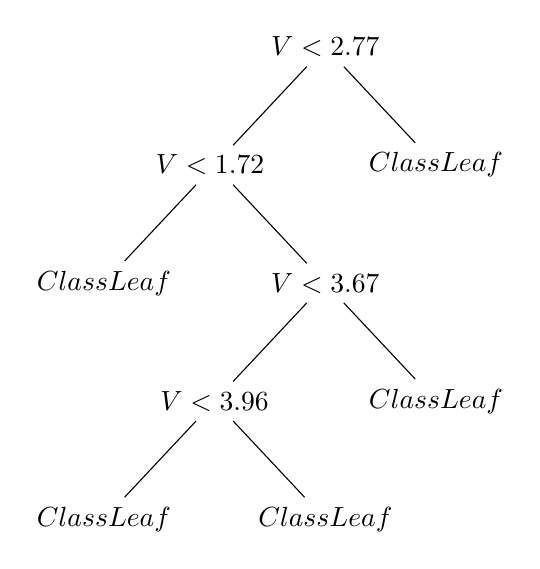
\begin{tikzpicture}[sibling distance=8em,
  every node/.style = {scale=1,
    draw=none, align=center}]]
  \node {$V < 2.77$}
 	  child { node {$V < 1.72$ }
 	    child { node {$Class Leaf$}}
 	    child { node {$V < 3.67$}
 	      child { node {$V < 3.96$}
 	        child { node {$Class Leaf$} }
 	        child { node {$Class Leaf$} }
 	      }
 	      child { node {$Class Leaf$} }
 	    }
 	  }
 	  child { node {$Class Leaf$} }
    ;
\end{tikzpicture}
\ \\
\begin{multicols}{2}
[Soit d'une façon plus calculatoire:
]
\begin{description}
\item[$G$] $=$
\item[] $left(X1_1) * (1 - left(X1_1))$ + 
\item[] $right(X1_1) * (1 - right(X1_1))$ + 
\item[] $left(X1_2) * (1 - left(X1_2))$ + 
\item[] $right(X1_2) * (1 - right(X1_2))$ + 
\item[] $left(X1_3) * (1 - left(X1_3))$ + 
\item[] $right(X1_3) * (1 - right(X1_3))$ + 
\item[] $left(X1_4) * (1 - left(X1_4))$ + 
\item[] $right(X1_4) * (1 - right(X1_4))$ + 
\end{description}

\begin{description}
\item[] $ $
\item[] $X1_1 = 2.77$
\item[] $ = 0$ car $V <$ 2.77 $\rightarrow$ Left
\item[] $ = 0$ car $1.72 <$ V $\rightarrow$ Right
\item[] $X1_2 = 1.72$
\item[] $X1_1 = 3.67$
\item[] $ = 0$ car $V <$ 3.67 $\rightarrow$ Left
\item[] $X1_1 = 3.96$
\item[] $ = 0$ car $V <$ 3.96 $\rightarrow$ Left
\end{description}
\end{multicols}
\pagebreak

\lstset{style=mlpythoncode}
\begin{lstlisting}[language=Python]
from sklearn.tree  import DecisionTreeRegressor

c = DecisionTreeRegressor().fit(xtrain,ytrain)
c.predict(xtest)
c.score(xtest, ytest)
\end{lstlisting}

\funcdoc{sklearn.tree.DecisionTreeRegressor}{}{}{
\begin{description}
\item[fit(X,y)] $\paramtype{pandas.DataFrame}$ Apprend le modèle avec les data $X$ et $y$.
\item[predict(X)] $\paramtype{pandas.DataFrame}$ Test l'apprentissage avec les données $X$ et retourne le $y$ généré.
\item[score(X,y)] $\paramtype{pandas.DataFrame}$ Retourne le coefficient de prédiction en comparent les $y$ généré avec le $y$ en paramètre.
\end{description}
}

\pagebreak
\section{K moyen}
Le K moyen demande une heuristique de type métrique pour comparé les distances entre poins.\\
Par exemple:
\begin{description}
\item[Distance euclidienne] $\sqrt{\sum_{i=1}^n (a_i, b_i)^2}$
\end{description}

\lstset{style=mlpythoncode}
\begin{lstlisting}[language=Python]
from sklearn.neighbors import KNeighborsClassifier 

c = KNeighborsClassifier(n_neighbors=2).fit(xtrain,ytrain)
c.predict(xtest)
c.score(xtest, ytest)
\end{lstlisting}

\funcdoc{sklearn.neighbors.KNeighborsClassifier}{
\begin{description}
\item[n\_neighbors] $\paramtype{Integer}$ le nombre de clusters
\end{description}}{}{
\begin{description}
\item[fit(X,y)] $\paramtype{pandas.DataFrame}$ Apprend le modèle avec les data $X$ et $y$.
\item[predict(X)] $\paramtype{pandas.DataFrame}$ Test l'apprentissage avec les données $X$ et retourne le $y$ généré.
\item[score(X,y)] $\paramtype{pandas.DataFrame}$ Retourne le coefficient de prédiction en comparent les $y$ généré avec le $y$ en paramètre.
\end{description}
}
\pagebreak

\section{Support vector machines}
\subsection{Margin classifier}
Soit les points:
\begin{description}
\item[$\cblue{Blue}$] Une $\cblue{ClassA}$
\item[$\crouge{Rouge}$] Une $\crouge{ClassB}$
\end{description}
Le support vector machines cherche un hyperplan (de couleur noir) pouvant départager les deux classes,
Il en existe une infinité d'hyperplan qui peuvent les départager, donc introduisons un autre concept, celui de 
l'hyperplan qui maximise la séparation entre les deux classes (les droites $\corange{Oranges}$ appelé $Margin$.\\

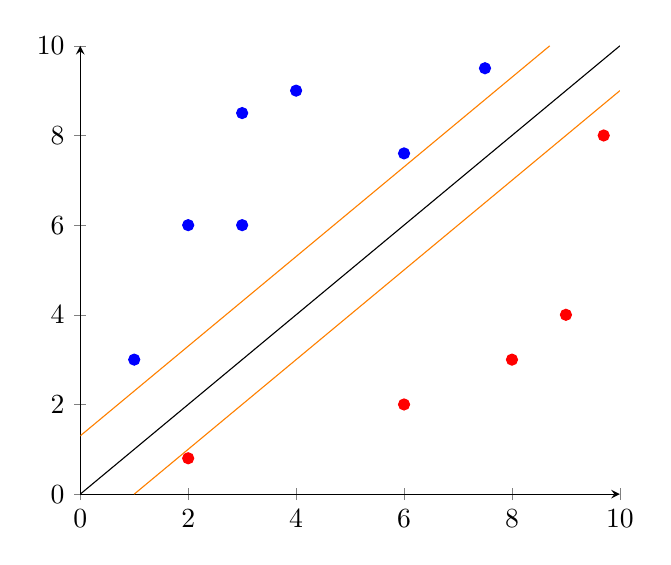
\begin{tikzpicture}
  \begin{axis} [
      axis lines = left,
      xmin       = 0,
      ymin       = 0,
    ]
    \addplot [color=black] coordinates {(0,0)(10,10)};
    \addplot [color=orange] coordinates {(0,1.3)(8.7,10) };
    \addplot [color=orange] coordinates {(1,0)(10,9) };
    \addplot [only marks, mark=*, color=blue] coordinates {(2,6)(1,3)(6,7.6)(3,8.5)(7.5,9.5)(4,9)(3,6)};
    \addplot [only marks, mark=*, color=red]  coordinates {(2,0.8)(6,2)(9,4)(9.7,8)(8,3)};
  \end{axis}
\end{tikzpicture}


\subsection{Soft margin classifier}
Dans le cadre du Soft margin, il n'existe pas de margin séparent les deux classes,il faut donc chercher la droite qui minimise l'erreur.
Soit un ensemble de données divisé en trois parties:
\begin{description}
\item[Tranning Set] sont les données qui seront utiliser pour l'apprentissage
\item[Test Set] les données qui sont utiliser pour vérifier la satisfesabilité de l'algorithme 
\item[Tunning Set] appeler $C$ qui sera le taux de violation de la margin accepté
\end{description}

Soit $C$ = $\{ 0.1, 1, 10\}$ les longueurs que peut prendre la margin et:\\
\begin{center}

\begin{tabular}{l|ll}
\hline
$ $ & $longeur\ de\ la\ margin$ & $F1\ Score$\\
\hline
$C_0$ & $0.1$ & 80$\%$ \\
$C_1$ & $1$ & 85 $\%$ La meilleur borne\\
$C_1$ & $10$ & 85 $\%$\\
\hline
\end{tabular}
\end{center}

\lstset{style=mlpythoncode}
\begin{lstlisting}[language=Python]
from sklearn.svm import SVC 

c = SVC().fit(xtrain,ytrain)
c.predict(xtest)
c.score(xtest, ytest)
\end{lstlisting}

\funcdoc{sklearn.svm.SVC}{}{}{
\begin{description}
\item[fit(X,y)] $\paramtype{pandas.DataFrame}$ Apprend le modèle avec les data $X$ et $y$.
\item[predict(X)] $\paramtype{pandas.DataFrame}$ Test l'apprentissage avec les données $X$ et retourne le $y$ généré.
\item[score(X,y)] $\paramtype{pandas.DataFrame}$ Retourne le coefficient de prédiction en comparent les $y$ généré avec le $y$ en paramètre.
\end{description}
}

\pagebreak